
Dado que el objetivo del trabajo es mejorar la asignaci\'on de momento para muones high-$p_{T}$, especialmente para los casos con showering, el primer aspecto que se ha de tener en cuenta es recopilar toda la informaci\'on posible del mu\'on (incluyendo los hits que provienen de las cascadas), en contraposici\'on a la estrategia de los distintos refits descritos en la Secci\'on~\ref{sec:current_assignment}, que tratan de encontrar aquellas c\'amaras donde es probable que haya tenido lugar una cascada para despu\'es eliminar la informaci\'on de dichas c\'amaras a la hora de hacer la reconstrucci\'on de la traza del mu\'on.

De esta manera, el procedimiento que se va a seguir para recoger toda la informaci\'on posible es extrapolar la traza del mu\'on medida en el tracker a las c\'amaras de muones, para despu\'es recoger todo el conjunto de hits que se encuentren en torno al punto extrapolaci\'on recogiendo as\'i todas las se\~nales que produzca la posible cascada. \\

En la presente secci\'on se detallar\'an las herramientas y metodolog\'ia utilizadas para el tratamiento de los datos.


\subsection{Herramientas utilizadas para el an\'alisis}\label{sec:tools}

Las herramientas utilizadas en el proceso de an\'alisis de los datos son las siguientes:

\begin{itemize}

\item CMSSW~\cite{cmssw} es una colecci\'on de software abierto utilizado principalmente para la hacer simulaci\'on, calibraci\'on, alineamiento, y reconstrucci\'on de objetos f\'isicos para el posterior an\'alisis de los datos. Para este trabajo se ha creado un c\'odigo en C++ que puede encontrarse en el repositorio~\cite{analyzer}. Este c\'odigo usa los m\'odulos de CMSSW para hacer la selecci\'on de muones y segmentos que se describir\'a en la secci\'on~\ref{sec:selection}. 

\item ROOT~\cite{root} es el marco de trabajo m\'as utilizado f\'isica de altas energ\'ias para el procesado de datos, an\'alisis estad\'istico, y herramientas de visualizaci\'on y almacenamiento de los datos. ROOT est\'a basado en programaci\'on orientada a objetos y escrito en C++, y se usar\'a como formato de los datos de entrada y salida del c\'odigo de selecci\'on~\cite{analyzer}.

\item Pandas~\cite{mckinney-proc-scipy-2010} (del ingl\'es \textit{Python Data Analysis Library}), es una librer\'ia de Python que ofrece gran rendimiento en el procesado de estructuras tabulares de datos. En este caso, se usar\'a Pandas, previa transformaci\'on de los datos en formato ROOT a csv, para el procesado de los segmentos seleccionados (operaciones de limpiado de segmentos, agregaciones, construcci\'on de las variables de entrenamiento...etc). Los m\'odulos creados para el procesado pueden encontrarse en \cite{processor}.

\end{itemize}


El proceso l\'ogico de trabajo en cuanto a las herramientas utilizadas y al formato de los datos se muestra en el siguiente diagrama de fases: 

\begin{center}
\smartdiagramset{border color=none,
   text width=3cm, font=\fontsize{10pt}{12pt}\selectfont,
   module x sep=4.0,     
   back arrow disabled=true}
\smartdiagram[flow diagram:horizontal]{Datos de simulaci\'on de entrada (formato ROOT),
  Selecci\'on de muones y segmentos (c\'odigo \cite{analyzer} en C++ con salida en formato ROOT),
  Tranformaci\'on de ROOT a texto (reader.py en \cite{processor}),
  Procesado de datos con Pandas: limpiado y construcci\'on de variables (doStep1.py y step2.py en \cite{processor})}
\end{center}


\subsection{Muestra de simulaci\'on utilizada}\label{sec:sample}

Se han generado 100000 eventos de $Z'$ con $m_{Z'}$ = 5000 GeV fruto de la colisiones prot\'on-prot\'on a una energ\'ia de centro de masas de 13 TeV (condiciones actuales del acelerador LHC) mediante simulaci\'on de Monte-Carlo utilizando el programa MadGraph5~\cite{Alwall:2014hca}. Se impone que las part\'iculas $Z'$ generadas se desintegren a un par de muones $\mu^{+}\mu^{-}$ y se simula el paso de los muones por el detector CMS con el paquete Geant4~\cite{Agostinelli:2002hh}. De esta manera se tiene una muestra con estad\'istica razonable de muones high-$p_{T}$ con $p_{T}$ generado conocido que se usar\'a para el entrenamiento de la DNN. \\

En la Figura~\ref{fig:data_pt} se muestran las distribuciones del $p_{T}$ generado y el $p_{T}$ proporcionado por el algoritmo TuneP de todos los muones de la muestra que pasan la selecci\'on detallada en la Secci\'on~\ref{sec:selection}.

\begin{figure}[h]
\centering
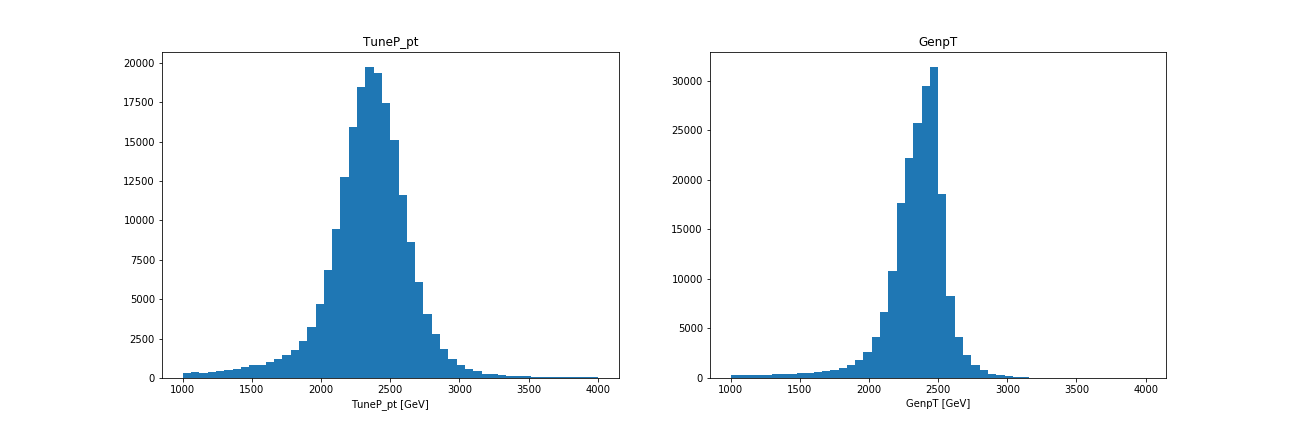
\includegraphics[width=1.0\textwidth]{figures/data_pt.png}
\caption{Distribuciones del momento transverso de los muones de la muestra de simulaci\'on utilizada. Izquierda: $p_{T}$ generado. Derecha: $p_{T}$ proporcionado por el algoritmo TuneP.}
\label{fig:data_pt}        
\end{figure}


\subsection{Selecci\'on de muones y segmentos}\label{sec:selection}

El proceso de selecci\'on de los muones y segmentos (ver c\'odigo \cite{analyzer}) de la muestra de Monte-Carlo para el posterior an\'alisis consta de las siguientes fases: 

\begin{enumerate}
\item Lectura de datos: En los datos de entrada, los muones y segmentos reconstruidos por evento se almacenan en colecciones de ROOT, que funcionan a modo de contenedor de informaci\'on. Por tanto el primer paso es leer las colecciones para poder iterar sobre ellas. 
\item Se recorre la colecci\'on de muones y se seleccionan aquellos que cumplen con los requisitos recogidos en la Tabla~\ref{tab:muon_sel}. Se pide que los muones tengan traza reconstruida en el tracker con $p_{T} >$ 200 GeV, y que esta traza reconstruida est\'e pr\'oxima a la traza generada del mu\'on dentro de un cono $\Delta$R = $\sqrt{(\Delta\eta^{2}+\Delta\phi^{2})} <$  0.3.
\item Posteriormente, se recorren todos los segmentos en el evento, y se almacenan sus coordenadas y los detectores en los que se encuentran si cumplen los requisitos registrados en la Tabla~\ref{tab:segment_sel}. B\'asicamente, se pide que los segmentos sean v\'alidos y se hayan medido correctamente sus coordenadas.
\item Se selecciona el estado m\'as externo de la traza del tracker y se extrapola (siguiendo la trayectoria de la traza y teniendo en cuenta el momento magn\'etico del solenoide de CMS) a la superficie de cada uno de los detectores guardados donde se ha encontrado al menos un segmento.
\item Se seleccionan aquellas extrapolaciones que cumplen los cortes de la Tabla~\ref{tab:prop_sel}. Se pide que las extrapolaciones sean v\'alidas, vayan en la direcci\'on del momento, y que la distancia entre el centro de la c\'amara y la extrapolaci\'on sea menor del tamaño de la c\'amara. Este \'ultimo requerimento es muy importante porque las superficies a las que se extrapola son planos de dimensi\'on infinita, y una part\'icula cargada que se curva debido a un campo magn\'etico siempre puede cortar un plano de dimensi\'on infinita.
\item Se guardan todas las variables almacenadas como objetos de ROOT, es decir, la informaci\'on sobre la traza del tracker, las coordenadas de los segmentos recogidos, y las coordenadas de las extrapolaciones.
\end{enumerate}

\begin{table}[htbp]
  \begin{center}
    {\normalsize
      \begin{tabular} {lc}
        \hline
        \hline
        Variable & Selecci\'on \\
        \hline
        TrackerTrack                          & Non-Null      \\
        TrackerTrack $p_{T}$ [GeV]            & $>$ 200       \\
        $\Delta$R(genMuon, recoMuon)          & $<$ 0.3       \\
        \hline
      \end{tabular}
    }
    \caption{Selecci\'on aplicada sobre la colecci\'on de muones, donde $\Delta$R = $\sqrt{(\Delta\eta^{2}+\Delta\phi^{2})}$ se calcula entre la colecci\'on de muones reoonstruidos y la colecci\'on de part\'iculas generadas.}
    \label{tab:muon_sel}
  \end{center}
\end{table}


\begin{table}[htbp]
  \begin{center}
    {\normalsize
      \begin{tabular} {lc}
        \hline
        \hline
        Objeto & Selecci\'on \\
        \hline
        SegmentoDT            & isValid()==1      \\
        SegmentoDT            & hasPhi()==1       \\
        SegmentoDT            & (hasZ()==1 or station==4)   \\
        SegmentoCSC           & isValid()==1      \\
        \hline
      \end{tabular}
    }
    \caption{Selecci\'on aplicada sobre la colecci\'on de segmentos.}
    \label{tab:segment_sel}
  \end{center}
\end{table}


\begin{table}[htbp]
  \begin{center}
    {\normalsize
      \begin{tabular} {lc}
        \hline
        \hline
        Objeto & Selecci\'on \\
        \hline
        Propagaci\'on          & isValid()==1                                                                 \\
        Propagaci\'on          & Hacia delante                                                                \\
        Propagaci\'on          & dist(extrapolaci\'on, centro de c\'amara) $\leq$ tama\~no de c\'amara      \\
        \hline
      \end{tabular}
    }
    \caption{Selecci\'on aplicada sobre las propagaciones. ``dist'' hace referencia a la distancia eucl\'idea.}
    \label{tab:prop_sel}
  \end{center}
\end{table}




\subsection{Procesado y construcci\'on de variables}\label{sec:procesado}

Como se ha mencionado en la secci\'on anterior, las propagaciones se hacen a planos de dimensiones infinitas, y a pesar de la selecci\'on en distancia de la Tabla~\ref{tab:prop_sel} a\'un se tienen algunas extrapolaciones que caen en agujeros o fuera de los l\'imites espaciales de CMS. En primera aproximaci\'on, para un mejor limpiado, se han definido circunferencias conc\'entricas en el plano xy, con radio Rxy en cent\'imetros, para limpiar la gran mayor\'ia de estas extrapolaciones. 

Una extrapolaci\'on en las DTs es eliminada del conjunto de datos si (Rxy$>$810.) \'o (Rxy $>$ 470. y Rxy $<$ 490.) \'o (Rxy $>$ 555. y  Rxy $<$ 590.) \'o (Rxy $>$ 670 y Rxy $<$ 690.); mientras que si se encuentra en las CSCs, se elimina si Rxy$>$720. En las Figuras~\ref{fig:segments_pos} y \ref{fig:props_pos} se muestran las posiciones espaciales de los segmentos y la propagaciones en los planos xy y xz una vez realizado el limpiado. \\


\begin{figure}
\centering
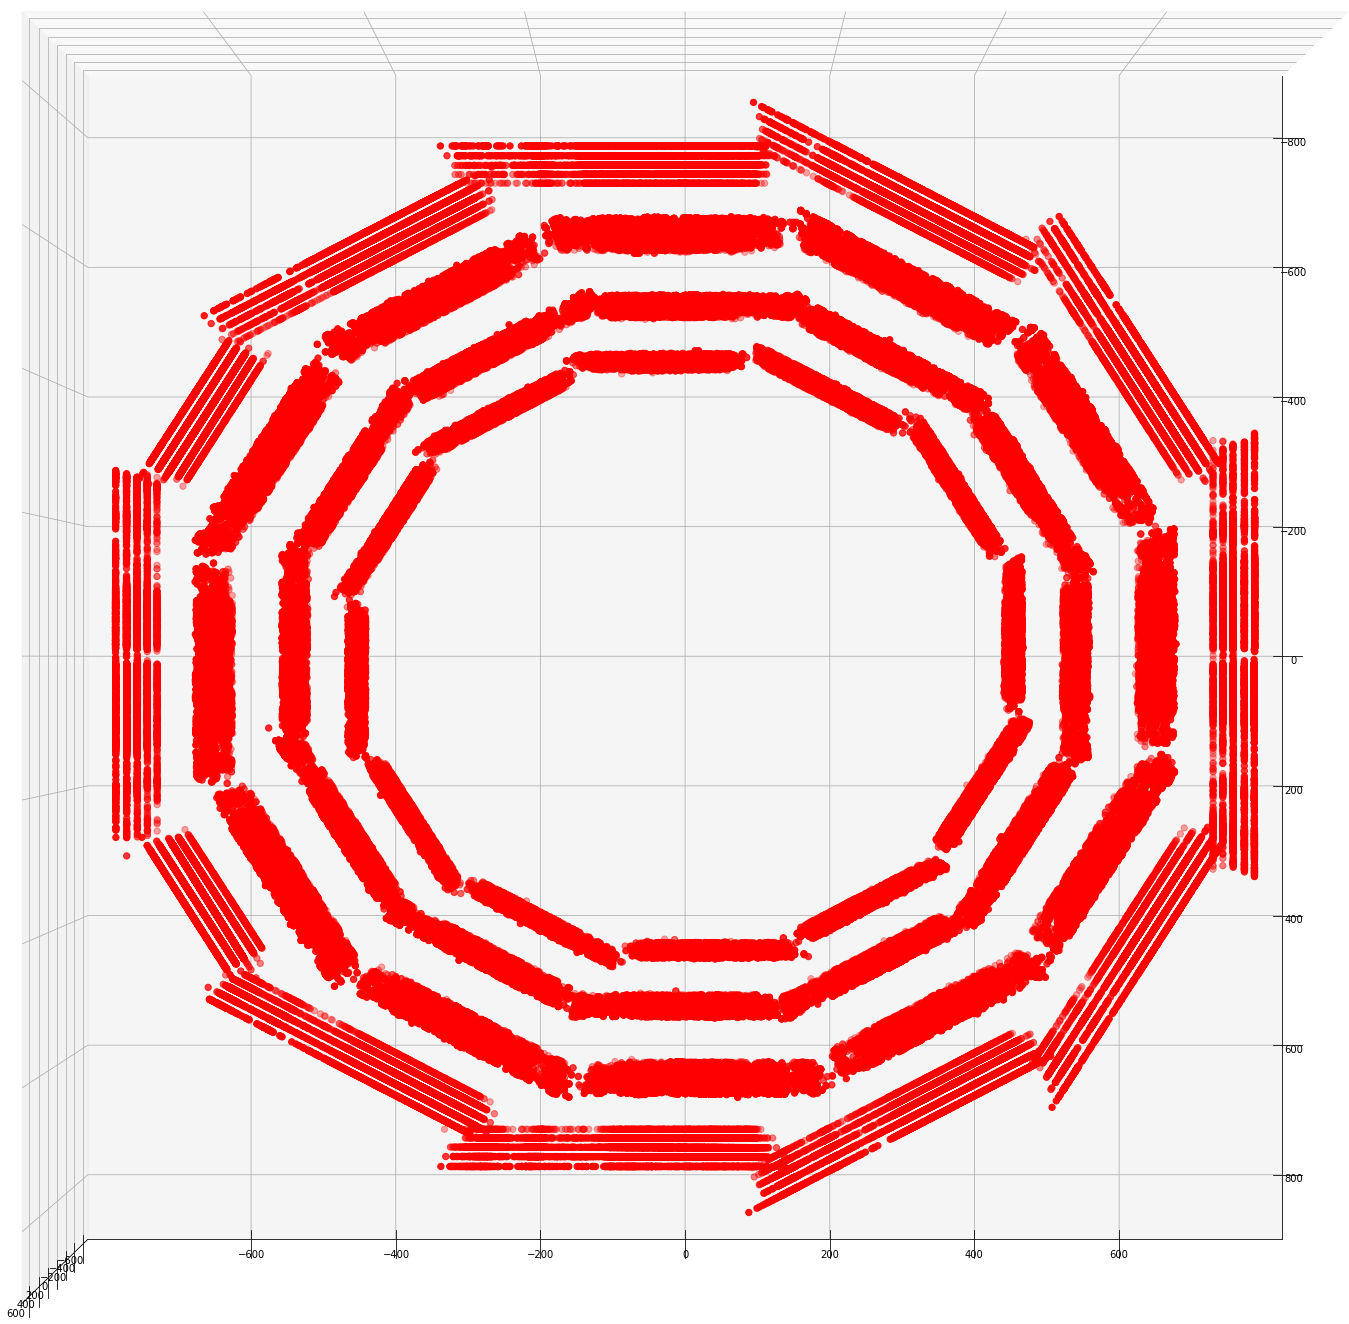
\includegraphics[width=0.4\textwidth]{figures/Hits_DT_xy_postCleaning.png}
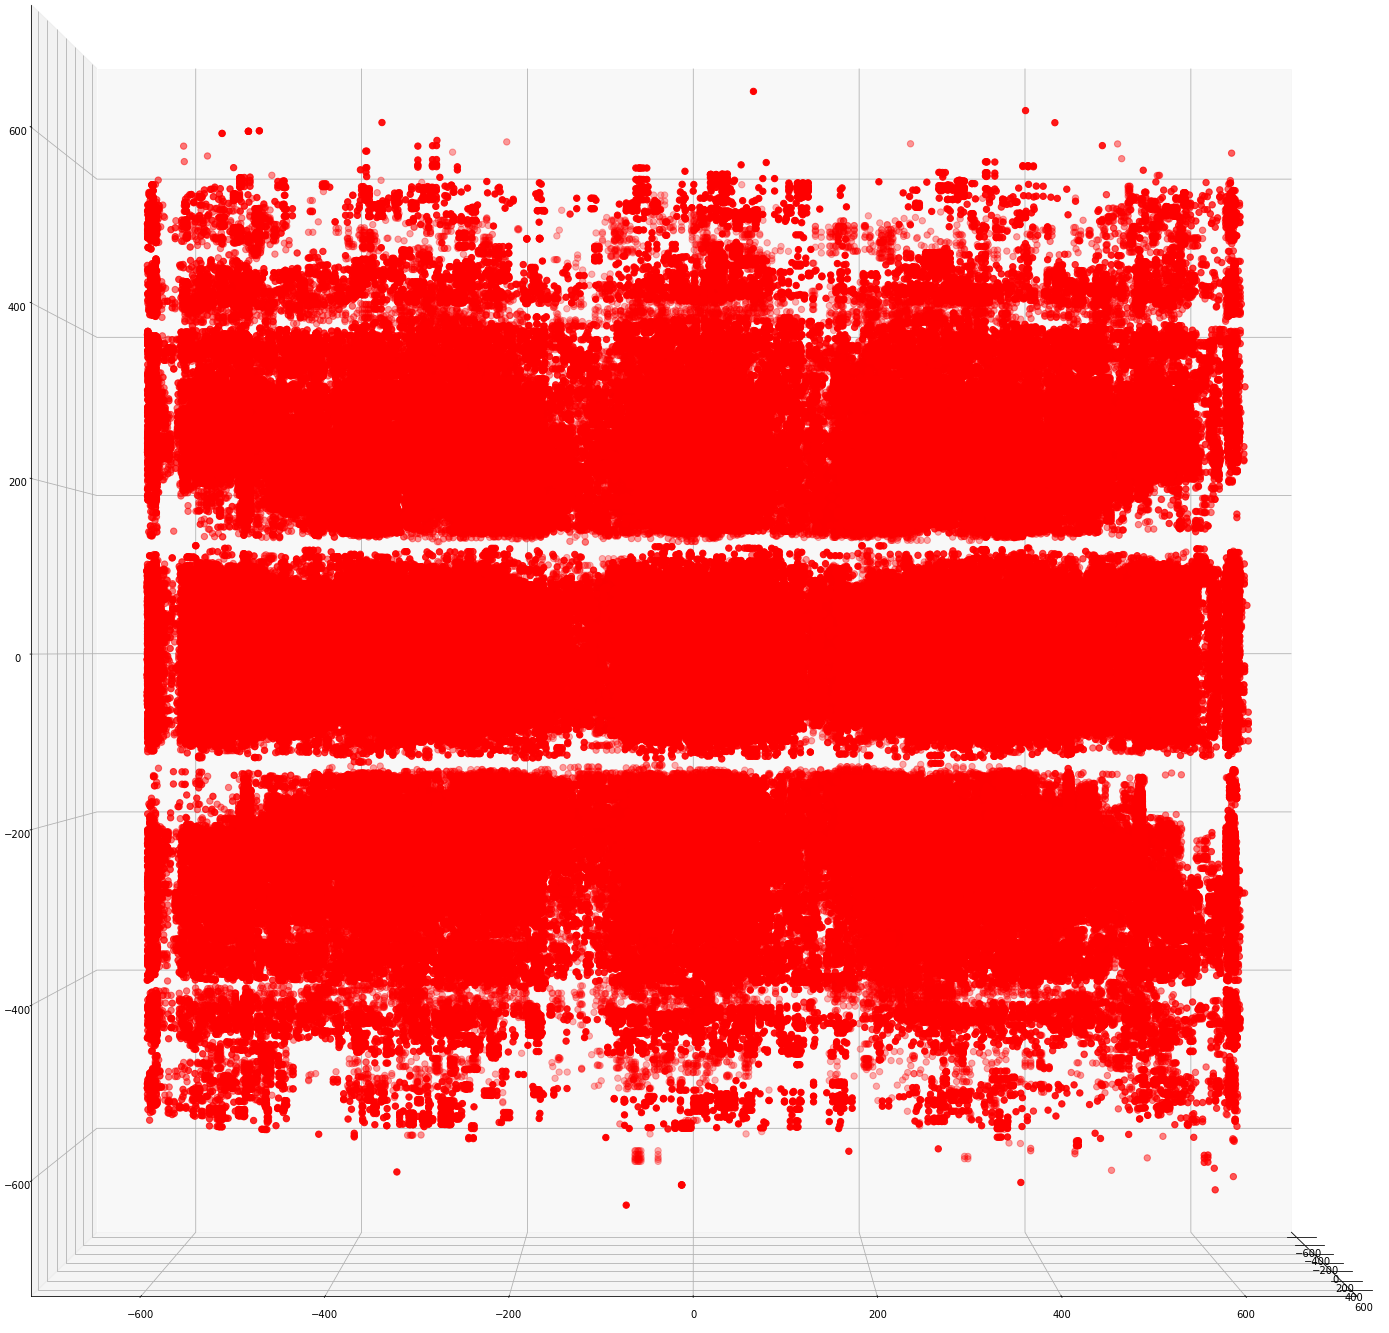
\includegraphics[width=0.4\textwidth]{figures/Hits_DT_xz_boarders.png}
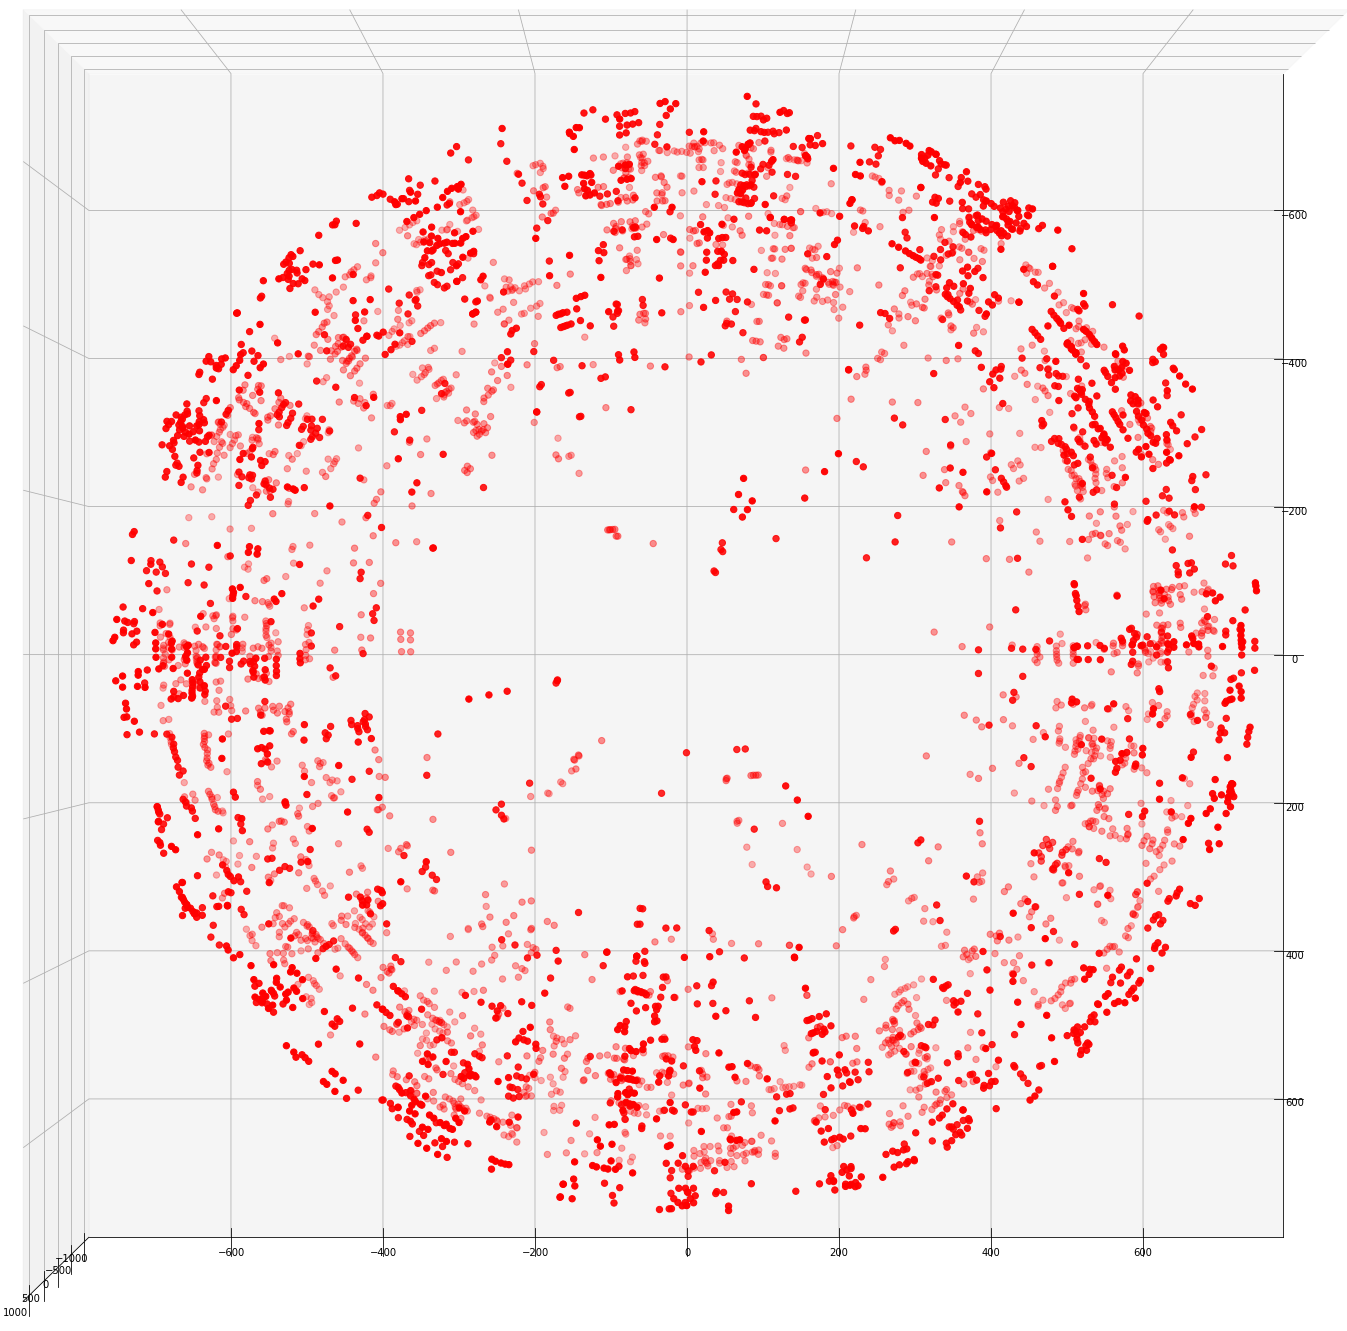
\includegraphics[width=0.4\textwidth]{figures/Hits_CSC_xy_boarders.png}
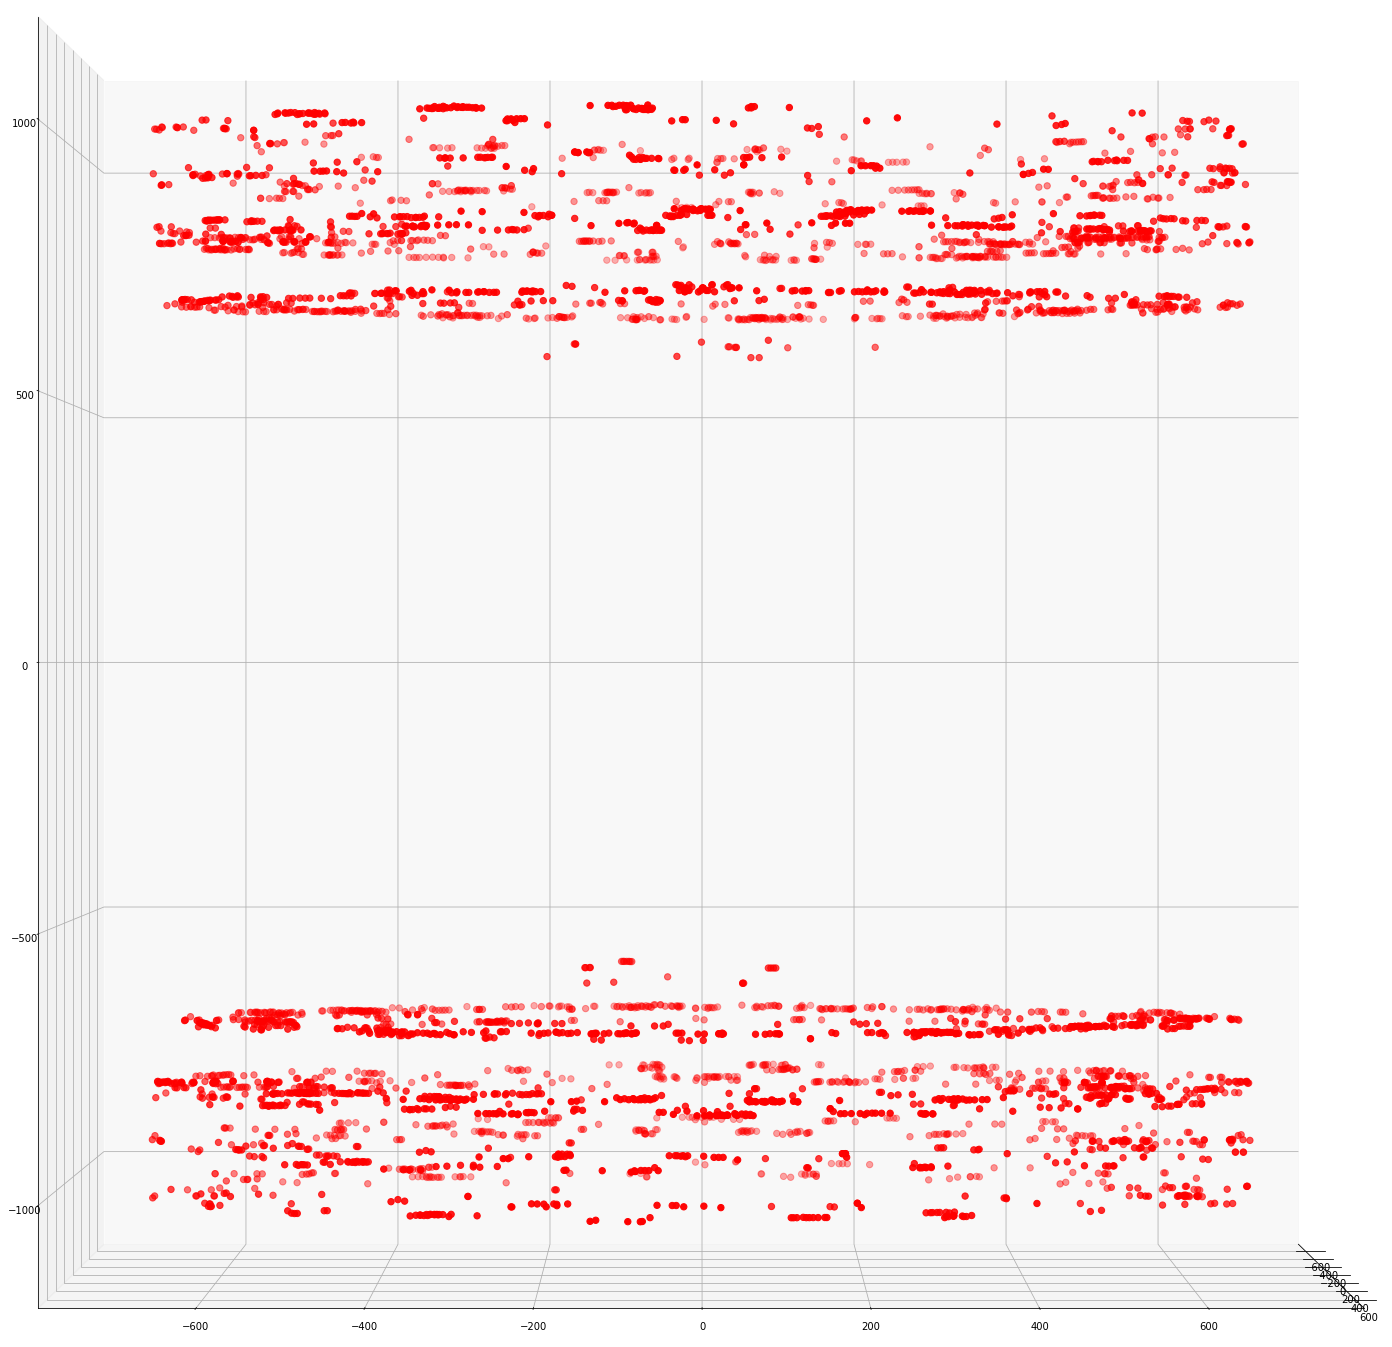
\includegraphics[width=0.4\textwidth]{figures/Hits_CSC_xz_boarders.png}
\caption{Posiciones geom\'etricas de todos los segmentos seleccionados. Arriba izquierda: Segmentos en DTs en el plano xy. Arriba derecha: Segmentos en DTs en el plano xz. Abajo izquierda: Segmentos en CSCs en el plano xy. Abajo derecha: Segmentos en CSCs en el plano xz.}
\label{fig:segments_pos}
\end{figure}


\begin{figure}
\centering
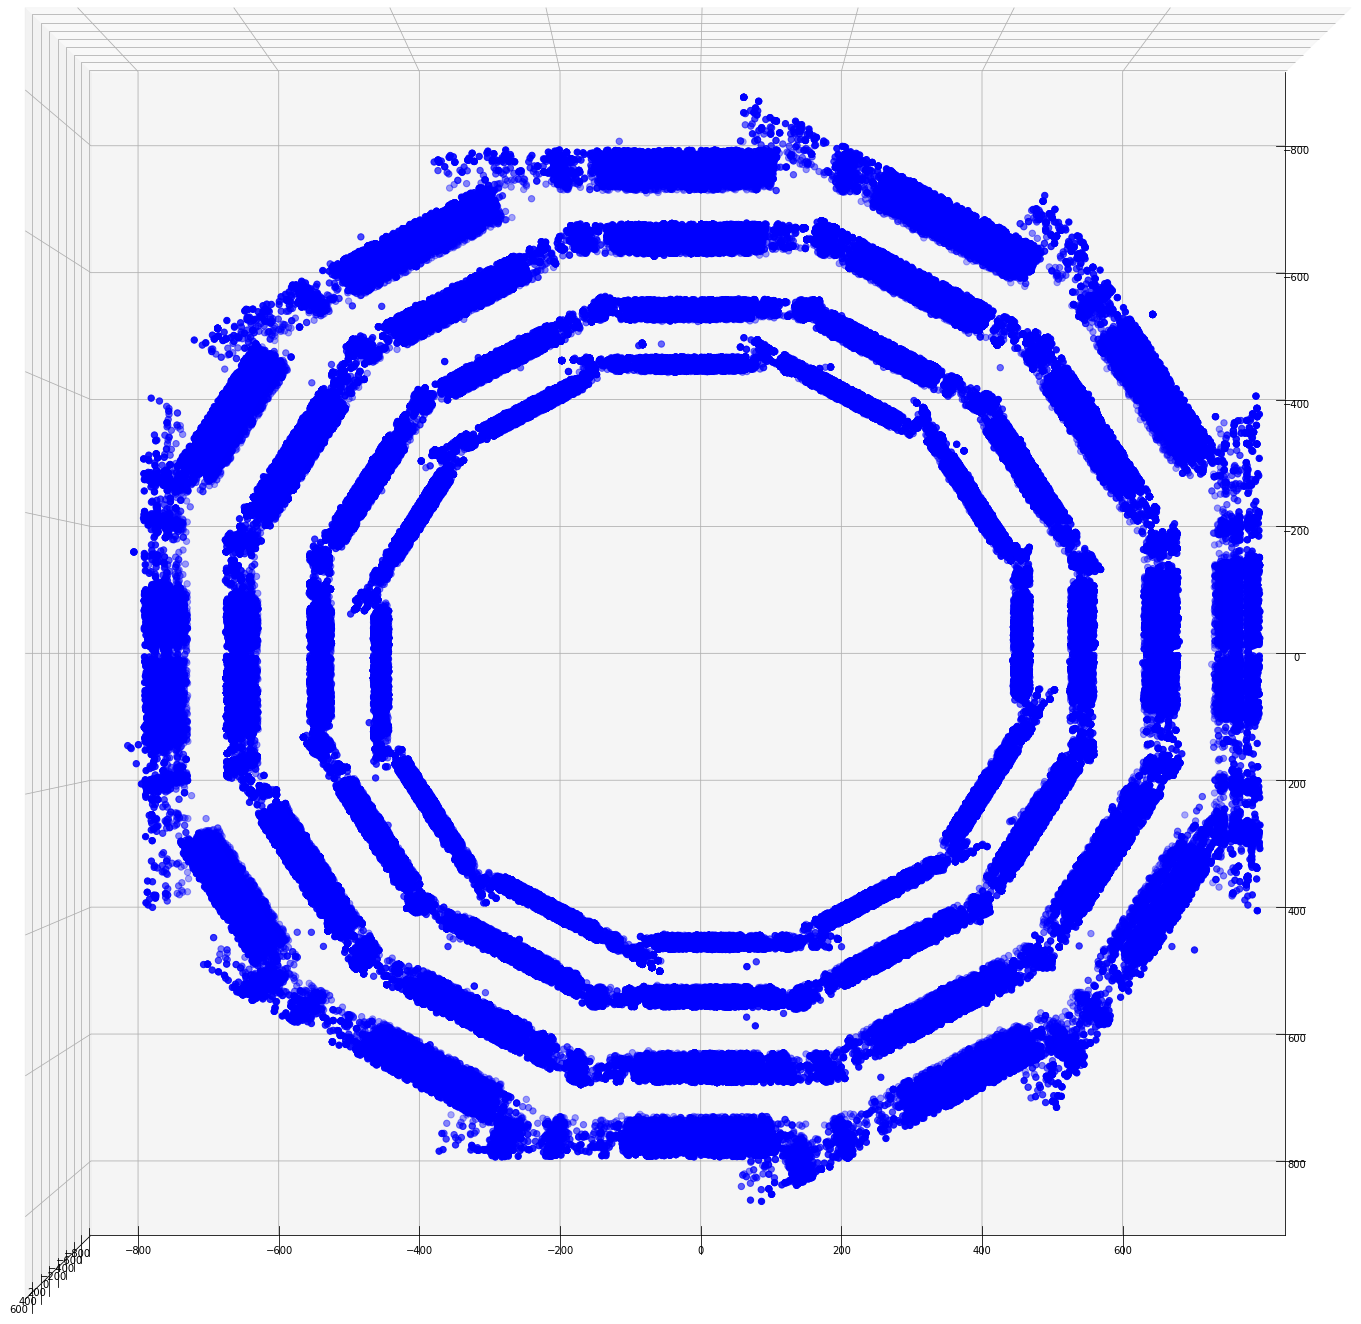
\includegraphics[width=0.4\textwidth]{figures/Props_DT_xy_postCleaning.png}
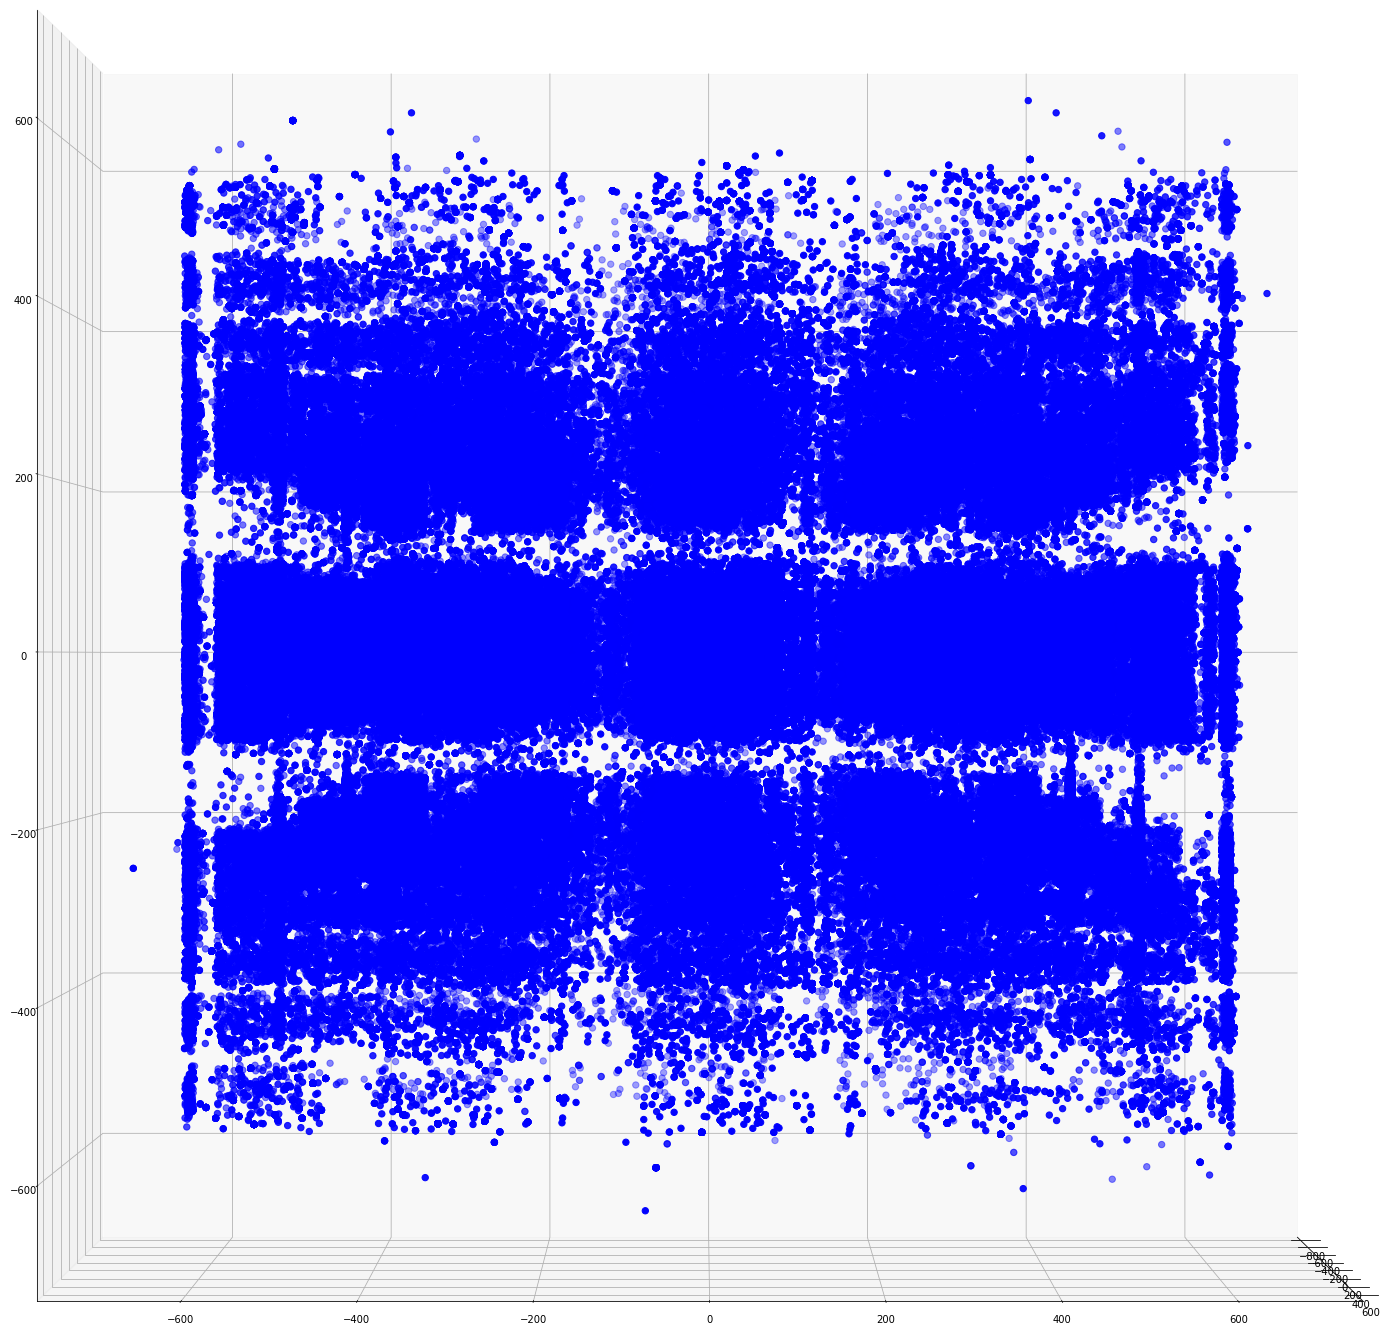
\includegraphics[width=0.4\textwidth]{figures/Props_DT_xz_boarders.png}
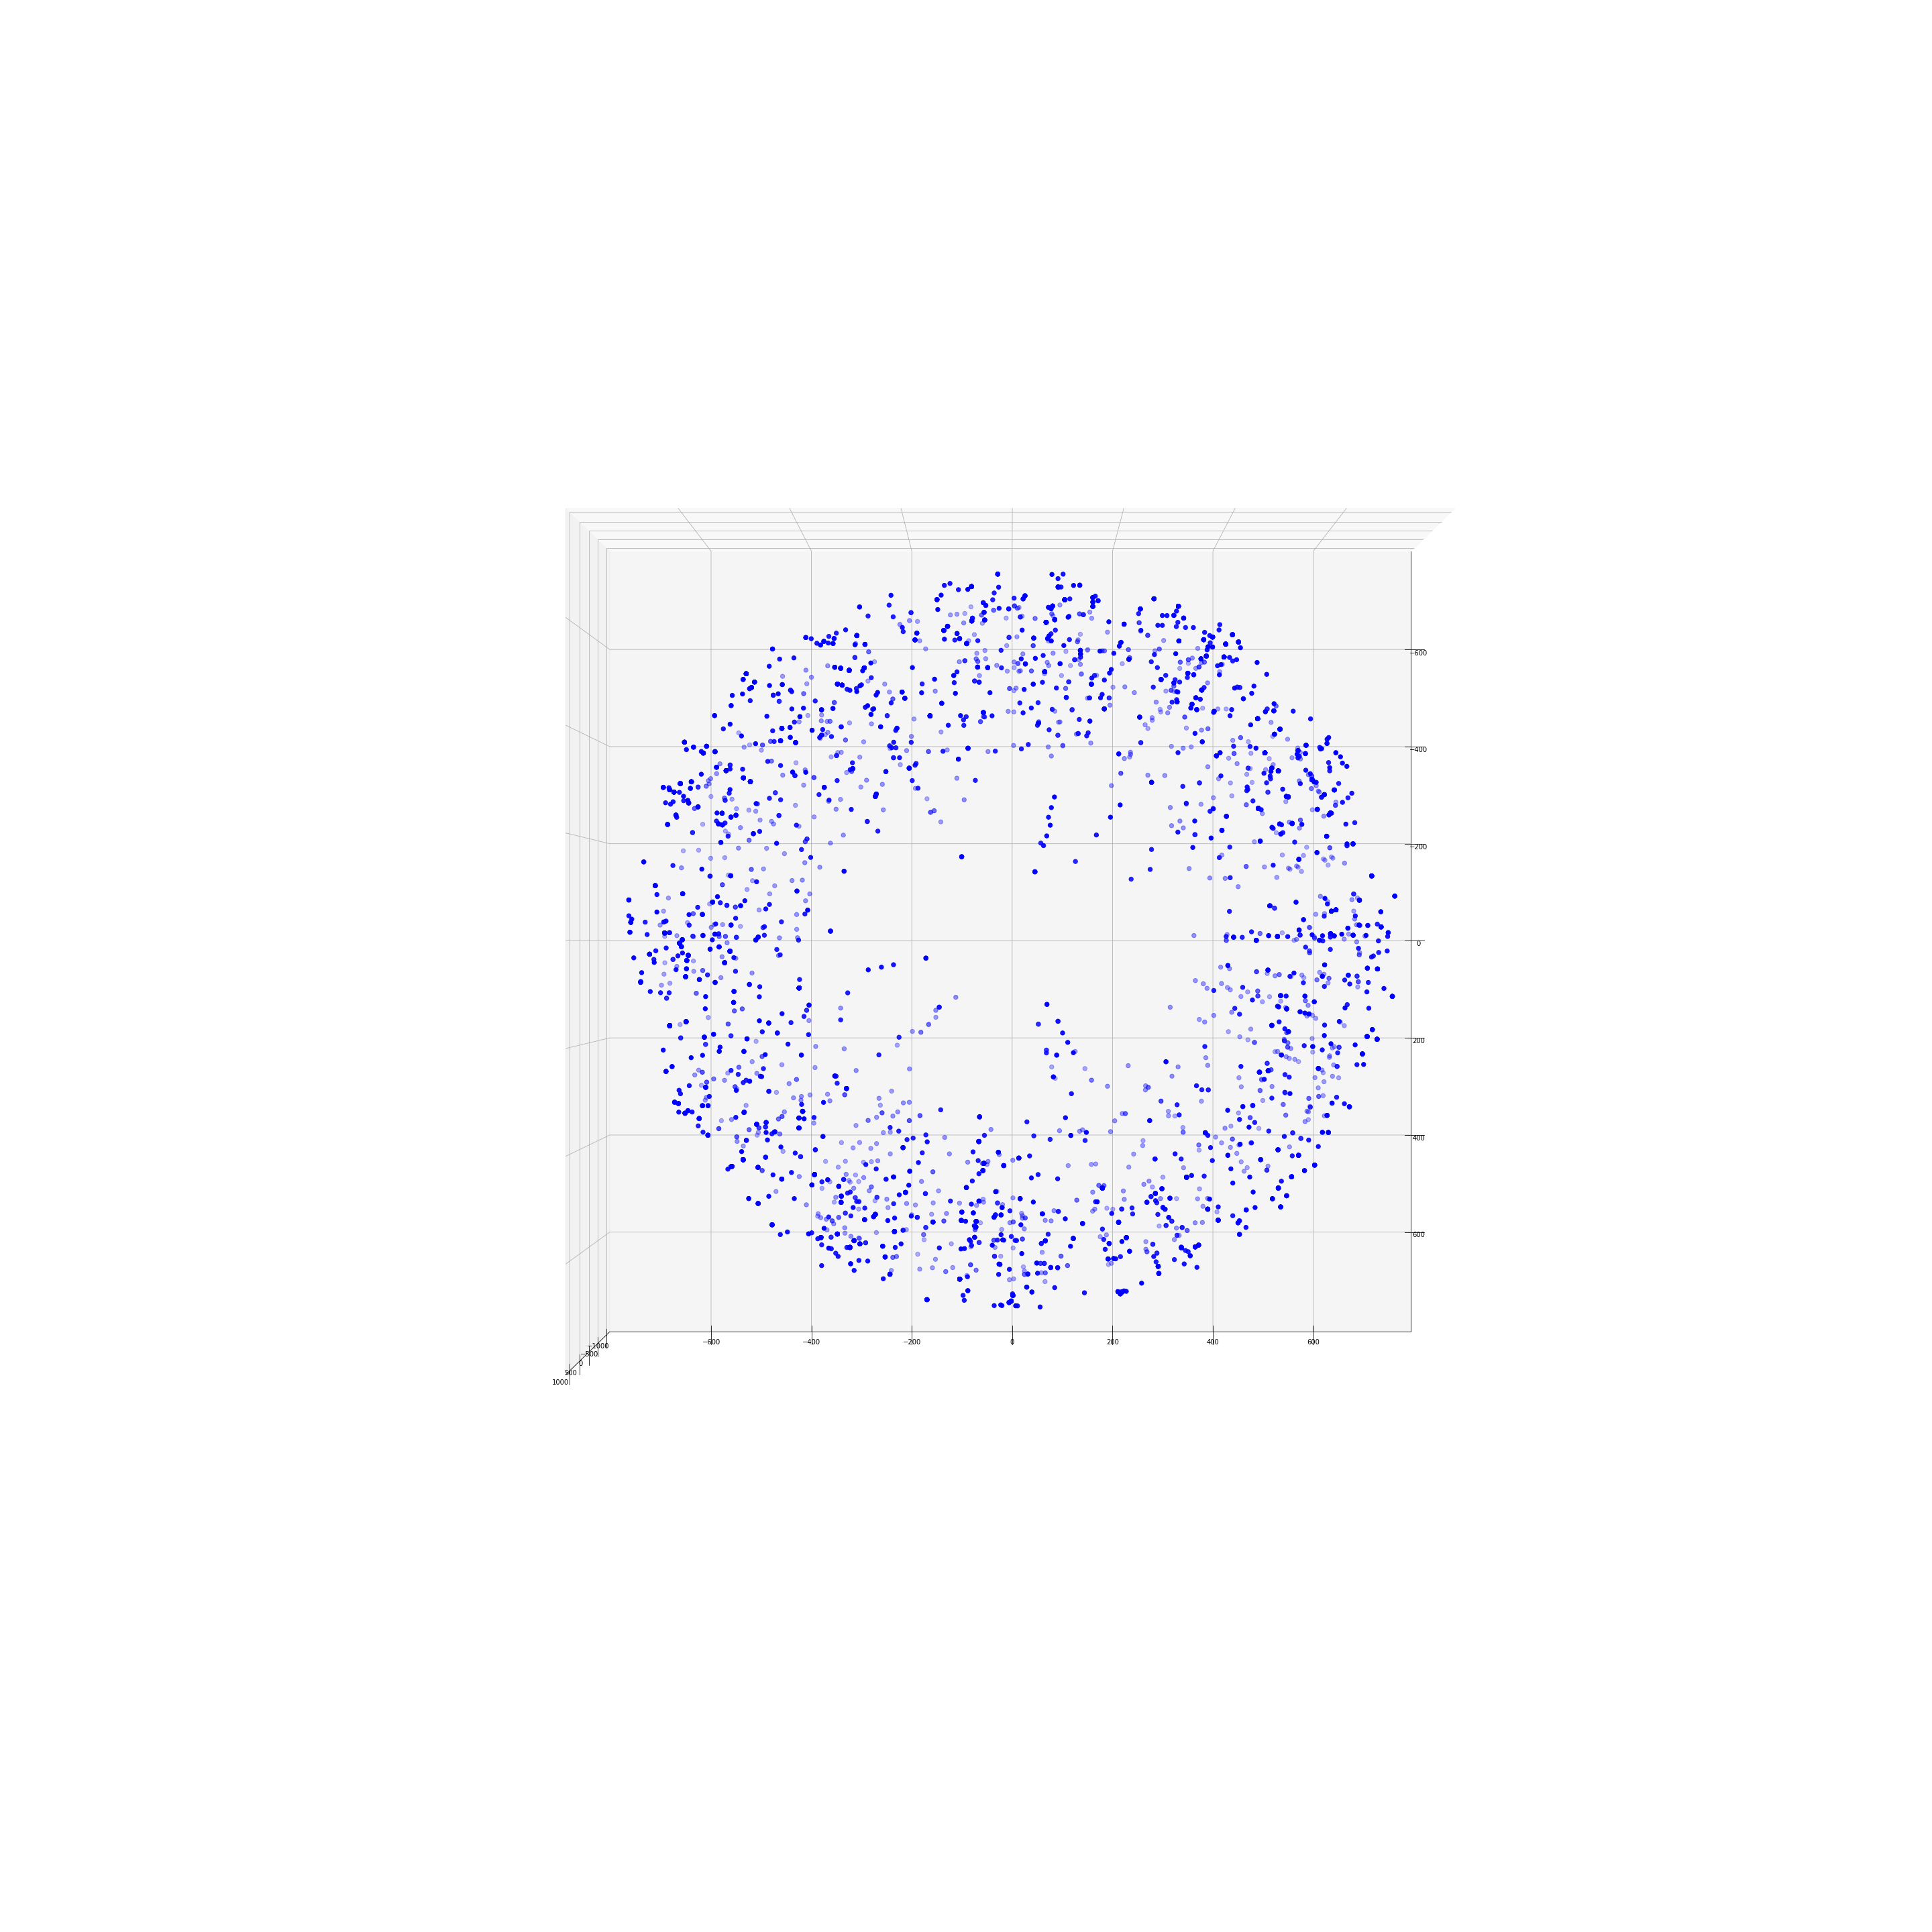
\includegraphics[width=0.4\textwidth]{figures/Props_CSC_xy_boarders.png}
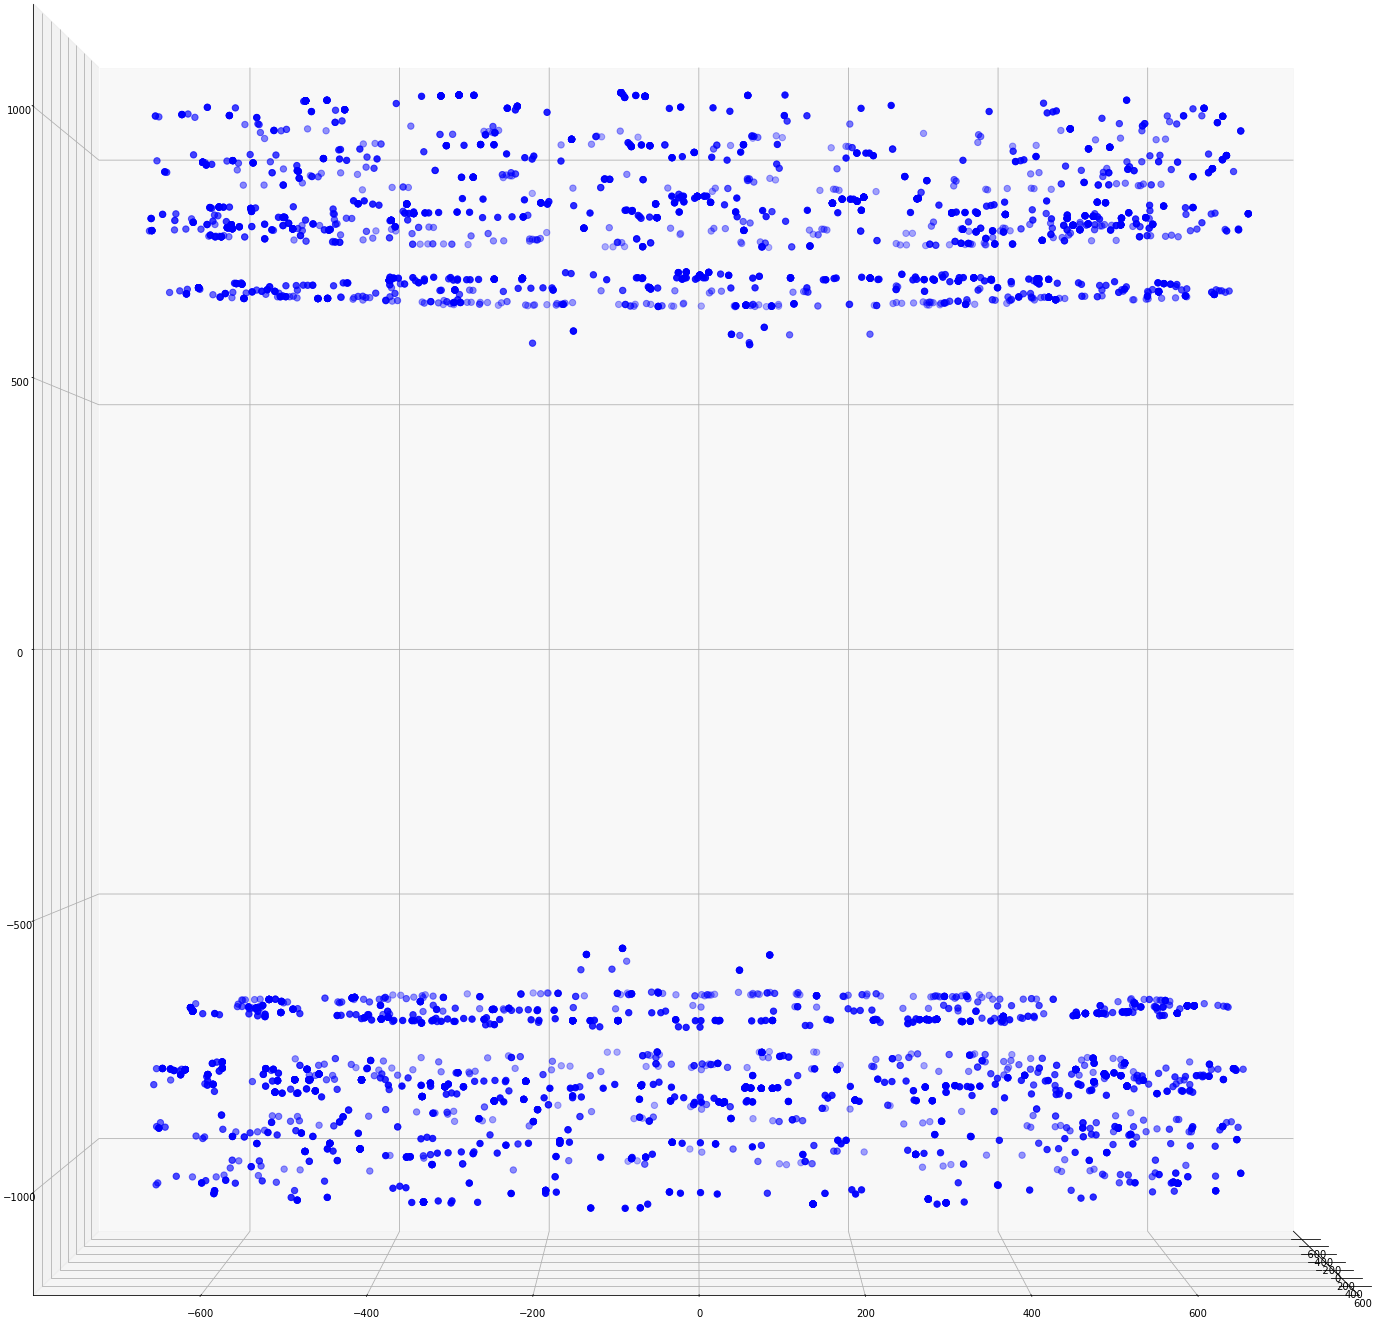
\includegraphics[width=0.4\textwidth]{figures/Props_CSC_xz_boarders.png}
\caption{Posiciones geom\'etricas de todos los propagaciones seleccionados. Arriba izquierda: Propagaciones en DTs en el plano xy. Arriba derecha: Propagaciones en DTs en el plano xz. Abajo izquierda: Propagaciones en CSCs en el plano xy. Abajo derecha: Propagaciones en CSCs en el plano xz.}
\label{fig:props_pos}
\end{figure}

Para la construcci\'on de las variables que ser\'an utilizadas en el entrenamiento se usan agregaciones de Pandas (ver doStep1.py en \cite{processor}). De esta manera, para cada mu\'on se agregan los segmentos encontrados en cada estaci\'on de DT y CSC y se obtiene el n\'umero de segmentos en cada estaci\'on, la media espacial de los segmentos, la distribuci\'on est\'andard, la asimetr\'ia y la kurtosis.



\subsection{Distribuciones de control}\label{sec:plots}

Se han realizado varias comprobaciones para asegurarnos que los datos tienen sentido. En primer lugar, se seleccionan muones con cuatro o m\'as segmentos en las DTs y adem\'as se require que tengan al menos un segmento en cada estaci\'on. Posteriormente, se separan los muones que cumplan estas condiciones en dos categor\'ias: aquellos que tienen exactamente cuatro segmentos (uno en cada estaci\'on), y aquellos que tienen m\'as de cuatro segmentos, donde los segmentos adicionales pueden provenir de cascadas. De esta manera, si para cada mu\'on se selecciona el m\'aximo valor de distancia entre el segmento y la propagaci\'on, uno esperar\'ia que la distribuci\'on de valores m\'aximos de distancias pique a valores m\'as bajos en la categor\'ia de cuatro segmentos que en la categor\'ia de m\'as de cuatro segmentos, y que se tenga una cola m\'as alargada en la segunda categor\'ia. Estas distribuciones se muestran en la Figura~\ref{fig:data_dist}. \\

\begin{figure}[h]
\centering
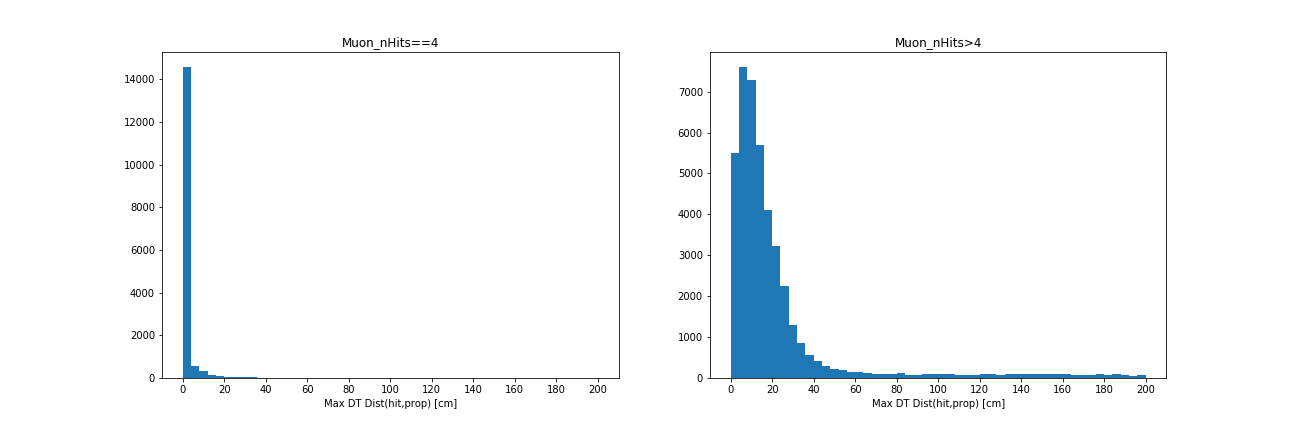
\includegraphics[width=1.0\textwidth]{figures/data_simple_dist_postCleaning.png}
\caption{Distribuciones del m\'aximo valor encontrado de distancia entre el segmento y la extrapolaci\'on (por mu\'on). Izquierda: Muones con cuatro segmentos en las DTs, uno en cada estaci\'on. Derecha: Muones con m\'as de cuatro segmentos en las DTs, y con al menos un segmento por estaci\'on.}
\label{fig:data_dist}        
\end{figure}


Por otra parte, en la Figura~\ref{fig:data_nSegmentsMean} se muestra la distribuci\'on de la media del n\'umero de segmentos por mu\'on en funci\'on del $p_{T}$ de generaci\'on. Se observa en este caso que hay una clara tendencia ascendente del promedio del n\'umero de segmentos con el $p_{T}$, ya que como se indic\'o en la secci\'on~\ref{sec:intro}, a mayor $p_{T}$ mayor es la probabilidad de que el mu\'on emita una cascada y se reconstruyan por tanto m\'as se\~nales en las c\'amaras.


\begin{figure}[h]
\centering
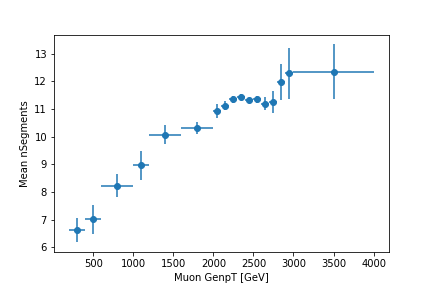
\includegraphics[width=0.5\textwidth]{figures/data_simple_genpt_MeanNSegments.png}
\caption{Distribuci\'on del promedio de segmentos encontrados por mu\'on en funci\'on del momento transverso generado.}
\label{fig:data_nSegmentsMean}        
\end{figure}
